\section{Results and Discussion}

Evolutionary innovations are adaptive traits that allow a lineage to cross a functional barrier and gain access to new niches. \cite{mayr1963animal} They are often framed as ``key innovations'' that can promote rapid diversification in the groups that evolve them \cite{heard1995key, hunter_key_1998}, and the search for key innovations has become a major component of modern macroevolutionary studies. \cite{maia_key_2013, rabosky_diversity-dependence_2013} However, despite the obvious importance of evolutionary innovations in the history of life on Earth, innovative traits rarely show a direct link with increased diversification. \cite{cracraft_origin_1990, vermeij_innovation_2001, vermeij_ecology_2007, vermeij_crucibles_2012, alfaro_does_2009, givnish_molecular_2000, hodges_spurring_1995, schluter2000ecology, brawand_genomic_2014, mitter_phylogenetic_1988}

Evolutionary innovations are also traditionally thought to reduce extinction rates, \cite{heard1995key} but this may not be the case if innovation facilitates the evolution of specialist phenotypes sensitive to ecological disturbance. \cite{futuyma_evolution_1988, givnish_adaptive_1998} Innovation may also exhibit niche-specific effects on extinction rates if the innovative trait involves a performance trade-off. \cite{schluter2000ecology} Specifically, performance may increase in new niches at the cost of competitive exclusion and eventual extirpation from previously accessible niches.

We examined the potential cost of evolutionary innovation by using a classic example: pharyngognathy. \cite{liem_evolutionary_1973} Pharyngognathy involves multiple modifications of the jaw apparatus in the back of the throat that allow a fish to generate high bite force, which likely enables pharyngognathous fishes to exploit hard-shelled and processing-intensive prey items. \cite{wainwright_biomechanical_1987} However, these modifications reduce pharyngeal gape, which may alter the maximum size of prey that can be easily swallowed. \cite{wainwright_evolution_2012}

Several lineages within the spiny-finned fishes have independently evolved pharyngognathy, including wrasses, surfperches, damselfish, marine halfbeaks, flyingfishes, and cichlids. \cite{wainwright_evolution_2012} Most of these lineages live in shallow marine habitats, except for cichlids, which occur mostly in tropical freshwaters. Cichlids are especially well known for their tendency to undergo rapid speciation and accumulate exceptionally large species richness in spatially confined assemblages, particularly in Lakes Victoria, Malawi, and Tanganyika in eastern Africa. \cite{greenwood1981haplochromine, seehausen2006african}

Each of these lineages has interacted with non-pharyngognathous spiny-finned lineages in different ways. In marine habitats, pharyngognathous lineages such as wrasses, parrotfishes and damselfishes have existed alongside closely related nonpharyngognathous spiny-finned fishes for tens of millions of years. \cite{wainwright_evolution_2012} In Lakes Victoria and Malawi, cichlids initially radiated in the complete absence of any nonpharyngognathous spiny-finned fish lineages. Unfortunately, in the 1950s, a nonpharyngognathous predatory fish, the Nile perch, Lates niloticus, was introduced into Lake Victoria, facilitating a cichlid mass extinction. \cite{witte_destruction_1992} In Lake Tanganyika, which hosts an older cichlid radiation than Victoria and Malawi, non-pharyngognathous Lates species and the pharyngognathous cichlids coexist, albeit with many fewer cichlid species and a lower speciation rate than the other two radiations. \cite{seehausen2006african, tiercelin1991lake}

Comparative dietary data reveal that pharyngognathy has ecological consequences for the marine lineages that possess the trait. Unlike cichlids, which can sometimes evolve into predatory niches free from competition with predators like Nile perch, marine pharyngognaths always occur alongside typical nonpharyngognathous fish-eating lineages. \cite{wainwright_evolution_2012} We surveyed diet data across a phylogeny of marine spiny-finned fishes, including four marine transitions to pharyngognathy as well as other spiny-finned species occurring in the same environments as those four lineages, and measured rates of dietary evolution for fish and processing-intensive prey like plants and hard-shelled animals. We analyzed diet both as a continuous character using Brownian motion and as a categorical variable using stochastic character mapping (see Methods). In both cases, we examined whether fishes with pharyngognathy had different rates of dietary evolution or rates of transition to a specialist diet for fish prey and processing-intensive prey. Pharyngognathous marine fishes evolved into niches favoring processing-intensive prey items at a much higher rate than other spiny-finned fishes (Figure \ref{FJ_fig1}). However, pharyngognaths evolved into fish-eating niches more slowly, suggesting that the evolution of the innovation may compromise access to this niche.

\begin{figure}
    \centering
    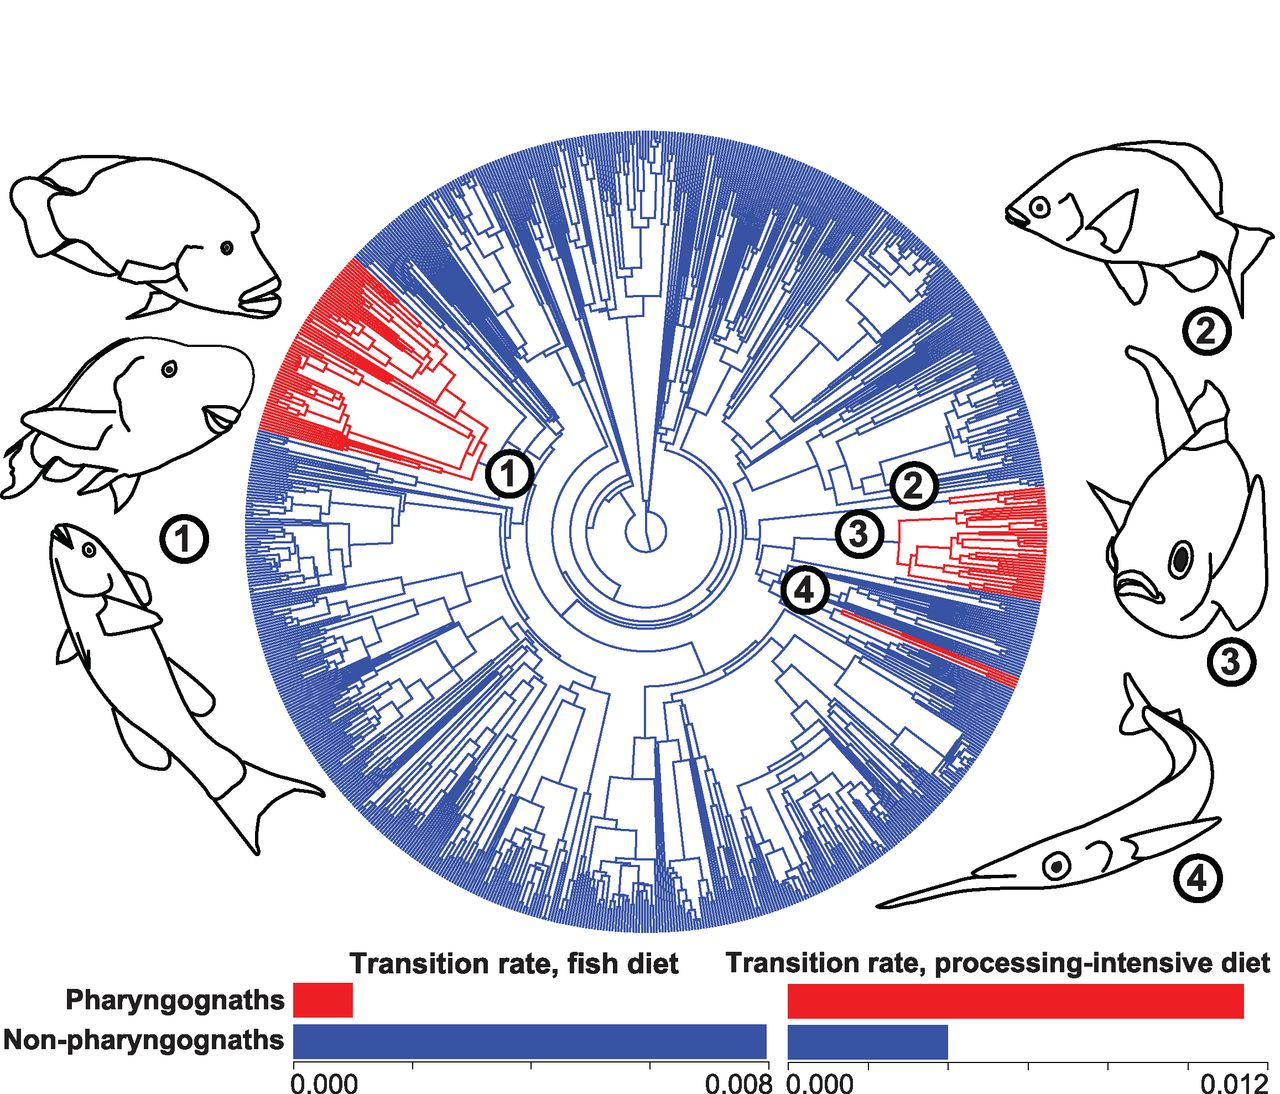
\includegraphics[width=\textwidth]{FishJaws/figures/fig1}
    \caption{\textbf{Pharyngognathy affects dietary transitions in marine fishes.} \textbf{(A)} Four transitions to pharyngognathy on a time-calibrated phylogeny of 851 marine spiny-finned fishes: (1) labroid fishes, including wrasses (Labridae), parrotfish (Scaridae), and weed whitings (Odacidae); (2) surfperches (Embiotocidae); (3) damselfishes (Pomacentridae); (4) marine halfbeaks (Hemirhamphidae). \textbf{(B)} Comparison of the transition rate for nonpharyngognathous and pharyngognathous fishes for fish prey and processing-intensive prey.}
    \label{FJ_fig1}
\end{figure}